

\chapter{Preliminaries}
\label{ch:preliminaries}

This section lists an overview of methods and concepts which are relied on in this work. The connection to the present work is briefly mentioned throughout the chapter.

\section{Recommender Systems}
Recommender systems are a class of information-retrieval systems that recommend items to users  \parencite{bobadilla2013recommender}. To generate individualized recommendations, they gather historical data of user-item interactions. In a video portal online setting, these could include explicit information such as user-item ratings and implicit information \parencite{bobadilla2013recommender} such as user clicks or the duration that users spent watching specific videos. Generally, RS use different approaches to generate recommendations \parencite{bobadilla2013recommender} such as: 

\begin{itemize}
    \item \textbf{Content filtering}-based approaches recommend items to a user based on the past interactions of the user with the items or similar items.
    \item \textbf{Demographic-based filtering} takes into account knowledge about personal attributes of the user such as age, gender, profession, or nationality.
    \item \textbf{Collaborative filtering}-based approaches recommend items to a user based on past interactions of a set of other users they consider similar to the first user. This approach is beneficial, because in real-world settings, user-item interaction data often is sparse, meaning that most users only interact with a small subset of all items. 
    \item \textbf{Knowledge Graph}-based approaches have gained popularity recently. KGs can provide additional side information to generate more accurate recommendations and add explainability to generated suggestions \parencite{guo2020survey}.
\end{itemize}


Real-world systems are often built as hybrid \parencite{bobadilla2013recommender} and will typically combine multiple different approaches to generate recommendations. 
Furthermore, these real-world settings can require the generation of recommendations for billions of users and millions of items in a small amount of time. Therefore, multistage RS are employed, which incorporate possible stages like the following \parencite{ma2020off}:

\begin{itemize}
    \item In the retrieval stage, a less precise system will retrieve a subset of candidate items from the set of all items.
    \item In the re-ranking stage, a more precise system will re-rank the retrieved subset of candidates to generate more accurate recommendations   
\end{itemize}


A common issue RS face is the cold-start problem \parencite{alyari2018recommender}, in which the system cannot identify well-suited candidate items or similar users for generating recommendations, because no or little data regarding the interaction of the user with the system have been collected yet.

\section{Mean Reciprocal Rank}
\begin{equation}
\text{MRR} = \frac{1}{|Q|} \sum_{i=1}^{|Q|} \frac{1}{\text{rank}_{i}}
\label{mrr}
\end{equation}


In the current work, the \ac{mrr} is used to evaluate the RS \eqref{mrr}. In the present case, given the ground-truth, the RS is scored by the rank of the item which they should recommend in first place among all other candidate items. If the \ac{rs} recommends the target item in fourth place, the reciprocal rank is $\frac{1}{4}=0.25$.  The reciprocal rank is then averaged over all queries in $Q$. This is a common evaluation approach \parencite{ying2018graph}, because it closely matches the goal of recommender systems, which is to recommend the correct items to users. Often users will only look at the first few items recommended to them. Therefore it is more important, which rank the correct item achieves in the first 30 positions, than it is important in the 1000 - 1030 positions. The MRR follows this rule.
\newpage
\section{Factorization Machines}
In this work, \acp{fm} \parencite{rendle2010factorization} are used as baseline to compare the proposed approach against. The top three contributions to the Netflix prize, from 2006 to 2009, include matrix factorization \parencite{freudenthaler2009factorization}. The Netflix challenge centered around the problem of predicting user ratings on a set of movies in the library of Netflix and popularized factorization approaches because of the winning contributions \parencite{freudenthaler2009factorization}. 

\begin{equation}
\min_{v_i*, v_u*} \sum(r_{ui} - v_u^T \cdot v_i)^2
 \label{eq:factor}
\end{equation}

According to \textcite{bokde2015matrix} the basic matrix factorization model maps users and items into the same vector space. The interest of a user with regards to an item is measured by the dot product between the user and item vector: $v_u^Tv_i$. These vectors can then be learned by minimizing the difference between the dot product and the known rating of users $u$ towards items $i$ for all know ratings $r_{ui}$ \eqref{eq:factor}. 

\begin{equation}
\hat{y}(\mathbf{x}) := w_0 + \sum_{i=1}^{n} w_i x_i + \sum_{i=1}^{n} \sum_{j=i+1}^{n} \langle v_i, v_j \rangle x_i x_j  \label{eq:fm}
\end{equation}
FMs \parencite{rendle2010factorization} use this method to learn a "general weight"  $\langle v_i, v_j \rangle$, capturing the pairwise interaction of the features in $\mathbf{x}$ \eqref{eq:fm}. 
In particular, besides $w_0 \in \mathbb{R}$ and $\mathbf{w} \in \mathbb{R}^n$ a matrix $\mathbf{V} \in \mathbb{R}^{n \times k}$ is learned containing $n$ vectors $v$ of dimensionality $k$, one for each feature, like an user or an item. This is beneficial when interaction data is sparse and a weight $w_{ij}$ is therefore not learnable as for example no interactions of user $i$ with item $j$ exist. By formulating $w_{ij}$ as the dot product of $v_i$ and $v_j$, both vectors can be learned independently through other observations $(y,\mathbf{x})$. An observation might be an event such as a user-rating $y$ towards a movie and the corresponding features of the user and movie $\mathbf{x}$.  The user and movie are dummy-encoded (The format is explained in Section \ref{sec:dataformats})  and concatenated forming the features of observation $\mathbf{x}$. The feature space can be expanded to other dimensions, such as "other movies rated", which can be dummy-encoded as well. Apart from this, the FM can model more complex interactions like 3-way interactions as well: $\langle v_i, v_j, v_k \rangle x_i x_j x_k$.




\section{Graphs}
In computer science, graphs can be regarded as data structures which can be used to describe real world networks, such as social networks \parencite{leskovec2008planetary}, traffic networks \parencite{derrow2021eta}, or they can represent abstract concepts such as joint graphs in human motion data \parencite{li2020dynamic}. Representing observations or modeling problems as graphs allows to formalize the problems and apply the theory and tools from the mathematical domain, where graphs can be represented as a set of vertices and edges. This allows to model social phenomena \parencite{leskovec2008planetary}, create more accurate weather predictions \parencite{khodayar2018spatio} or optimize traffic routes \parencite{derrow2021eta}. This thesis deals with a heterogeneous graph consisting of multiple entity and edge types. The present graph might be regarded as a Knowledge Graph, as it integrates a ``large cross-domain dataset'' \parencite{paulheim2017knowledge} from different sources and models the interrelation of facts \parencite{pujara2013knowledge}.

Following the formulation of \parencite{hu2020heterogeneous}, a heterogeneous graph can be expressed as 
$G = (\mathcal{V}, \mathcal{E}, \mathcal{A}, \mathcal{R})$,
where each node $v \in \mathcal{V}$ and each edge $e \in \mathcal{E}$ is mapped by mapping functions $\tau(v) : \mathcal{V} \to \mathcal{A}$ and $\phi(e) : \mathcal{E} \to \mathcal{R}$ to their respective node- and edge type. Each directed edge $e, \psi(e) = (s,t)$ has a corresponding meta relation $\langle \tau(s), \phi(e), \tau(t) \rangle$, which is the relation of the underlying node- and edge types. The degree of a node $v$ is the number of edges it has to other nodes in the graph.


Lastly, by choosing to model a network as graphs to solve a task, an inductive bias is introduced.  Furthermore, there exist different ways to represent the same network as a graph. The optimal representation can depend on the problem which has to be solved. For example, in the case of GNN-training, selected hyper-edges can be constructed which aid the learning process \parencite{yadati2019hypergcn}. 
\section{Data Formats}
\label{sec:dataformats}


\begin{equation}
    \mathbf{A}_{ij}  =\begin{cases} 
    1,& \text{if } (v_i,v_j) \in \mathcal{E}\\
    0              & \text{otherwise}
    \end{cases}
    \label{eq:adj}
\end{equation}



Sparse matrix representation allows to store and process matrices in a memory-efficient way. In graphs, the connectivity information can be represented using the adjacency matrix $\mathbf{A}^{n \times n}$ \eqref{eq:adj}, where $n$ represents the number of nodes in the graph. An undirected graph, where edges have no direction, is denoted with entries for edges in both directions in the adjacency matrix. 


The memory requirement to store these matrices grows quadratically with the number of nodes $n$, whereby loading these matrices into main memory to perform computations becomes infeasible. However, taking advantage of the fact that real world graphs are sparse, meaning $|\mathcal{E}| \ll |\mathcal{V}| \cdot (|\mathcal{V}| - 1)$, 
Adjacency matrices can be expressed as a $2 \times |\mathcal{E}| $ matrix. In detail, the matrix will contain a directed edge in both directions in place of the undirected edge, similar to the notation of the adjacency matrix.
\begin{equation}
C_{ij} = \sum_{k=1}^{n} A_{ik} \cdot B_{kj} \label{eq:matrix_mult}
\end{equation}


Matrix multiplication can be represented as a sum of products of the entries of the participating matrices \eqref{eq:matrix_mult} During computation, the zero entries can simply be ignored.
By using the sparse formulation, for the cost of computational overhead, matrix multiplication can be performed without the need to allocate memory for the whole adjacency matrix. Throughout this work, sparse matrices are utilized in the implementation of Graph Neural Networks as well as for feature engineering. Pytorch-sparse \parencite{pytorch_sparse} provides graphics-card accelerated sparse matrix-matrix multiplication for use in the programming language Python \parencite{python}.

  \begin{equation}
    c_4 = (0,0,0,1,0) \label{eq:dummy}
  \end{equation}
  
\textbf{Dummy encoding} can be utilized to encode non-continuous categorical data. In the example  \eqref{eq:dummy}, the variable $c$ has 5 values or categories. $c_4$ can be represented as shown. 

\section{Embeddings for Graphs}
In the Machine Learning domain embeddings are learned to compress information, such as of entities, into a vector space. Advancements in the \ac{nlp} domain such as Word2Vec \parencite{mikolov2013efficient} and GloVe \parencite{pennington2014glove} have shown the effectiveness of embeddings in the language domain. The embedding algorithms consider the co-occurrence of words in large corpora to condense information into vector representations of these words. These vector representations map the entities into a metric space, which allows to compare them numerically. Taking words as entities, semantically similar words obtain similar vector representations. 

\begin{equation}\label{eq:minkowski}
    d(u, v) = \left( \sum_{i=1}^{n} |u_i - v_i|^p \right)^{\frac{1}{p}}
\end{equation}

\begin{equation}\label{eq:cosine_similarity}
    \text{Cosine Similarity} = \frac{{u \cdot v}}{{\|u\| \|v\|}}
\end{equation}

Common measures include the Minkowski distance \eqref{eq:minkowski} and the cosine similarity \eqref{eq:cosine_similarity} where $||u|| = d(u,\mathbf{0})_{p=2}$. For example, the vector separating the embedding for “man” and “woman” is similar to the one separating “king” and “queen”, which can be interpreted as the “gender” component. This reveals the possibilities given by embeddings to reason in the embedding space. A later section introduces Knowledge Graph embeddings which build upon this intuition. For real-world application, the notion of learning embeddings can be extended to different modalities like images, documents to enable semantic search capabilities. 

Following the advancements in NLP, similar methods have been developed in the graph domain. Early methods such as DeepWalk \parencite{perozzi2014deepwalk} or Node2Vec \parencite{grover2016node2vec} focus on compressing structural information of the graph into embeddings. Node2Vec for example, similar to methods in the NLP domain, looks at co-occurences of nodes to generate their embeddings. The notion of co-occurence is defined by the simultaneous appearance of nodes in a fixed-size random walk on the graph starting from random seed nodes. Altering the parameters p and q changes the behavior of the "random walker" returning to the last node, staying at the same distance to the last node or proceeding further away from the last node. This allows to learn different structural information depending on chosen p and q. When the the breadth-first approach is chosen, more local information will be captured. The depth-first approach will capture more global neighborhood information.

\section{Knowledge Graph Embeddings}

There exist different methods such as DistMult \parencite{yang2014embedding}, ComplEx \parencite{trouillon2016complex} or TransE \parencite{bordes2013translating} to learn node embeddings in heterogeneous graphs (Figure \ref{fig:kge}). In detail, these methods try to learn the underlying relationships between entities. In this paper, TransE is combined with the HGT to learn node embeddings. 

\begin{figure}
    \centering
    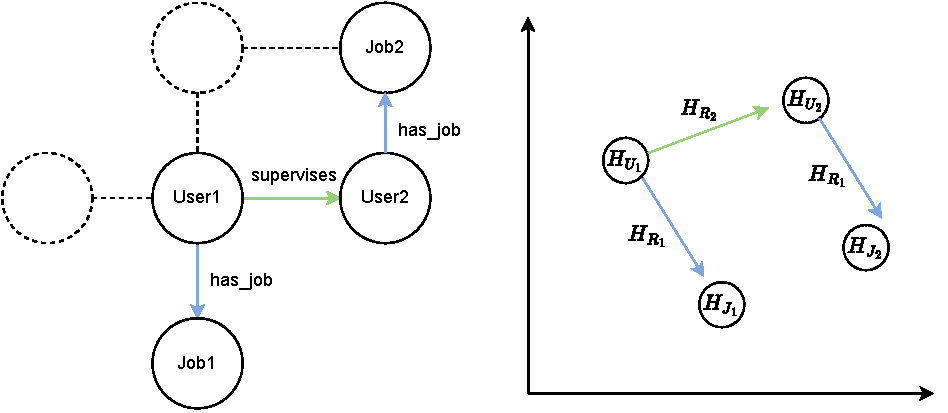
\includegraphics[width=0.8\textwidth]{img/kge.drawio (3).pdf}
    \caption[Learning node embeddings with TransE]{ Methods such as TransE map graphs into a metric space by learning node  and relationship embeddings.}
    \label{fig:kge}
   
\end{figure}
\begin{equation}
d(s,r,t) = - \| h_s + h_r -h_t \|_p
\label{eq:kge}
\end{equation}

TransE learns embeddings with the scoring function \eqref{eq:kge} such that given the edge $e, \, \psi(e)=(s,t), \, \phi(e)=r$, the embedding of node $s$, $h_s$ translated in space by the relationship-specific embedding $h_r$ is close to the embedding of node $t$, $h_t$., where  $\|... \|_p$ is the Minkowski distance. Embeddings can be learned from a random initialized lookup table and gradient descent, which the methods in the previous section use as well. Learning the relationship embeddings $h_r$ allows to apply reasoning in the embedding space. \textcite{ren2020query2box} illustrate this ability by the example of finding "Canadians which won the Turing-Award" by applying the corresponding relations "citizen" and "won" to the Canada and Turing-Award nodes to find nodes of citizens in the vicinity. The present work does not explore this dimension any further, but incorporates TransE to learn node embeddings. The example in Figure \ref{fig:kge} illustrates the need for methods like TransE, as without the relationship embeddings $h_r$ it becomes difficult to represent multiple relationship types and non-symmetric relationships in the same embedding space.  In theory, TransE can not model symmetric relationships well \parencite{sun2019rotate}, as only $h_r=\mathbf{0}$ could model such a relationship . The relationship of coworkers represents a symmetric relationship. However, TransE has been shown to still perform well despite its incomplexity when compared to more advanced methods \parencite{sun2019rotate}.



\section{Graph Neural Networks}
This section provides a brief overview over a selection of Graph Neural Network  architectures and illustrates how the training can be approached. 

Fundamentally, Graph Neural Networks are similar to the graph-based embedding methods introduced in the previous section, in that they can be utilized to compute node embeddings.  But they can be extended to edge- and graph-level tasks as well, incorporating node and edge features  and further considering different node and edge types such as present in heterogeneous graphs. Additionally, sampling methods have been developed \parencite{ying2018graph}, which allow the training of those networks on graphs with several billions of edges  using stochastic gradient descent. 
The present paper applies the Heterogeneous Graph Transformer (HGT) \parencite{hu2020heterogeneous} to a learning recommendation problem. 
The HGT builds up on several advancements in the field, introduced in the following paragraphs.


\begin{equation}
h_t^l = \sigma\left(   \sum_{s \in \mathcal{N}(t)} \frac{\mathbf{W}^l \cdot h_s^{l-1}}{|\mathcal{N}(t)|} \right) \label{eq:matrix_mult2}
\end{equation}

The concept of Graph Convolution is introduced by \textcite{kipf2016semi} with the \textbf{Graph Convolutional Neural Network} (GCN). Their initial formulation of the network considers the whole graph. This paper uses the node level formulation \eqref{eq:matrix_mult2} by the authors as the formulation is further extended upon.


The formula describes one layer $l$ of the GCN, specifically the computation of the node representation $h_t^l$ of node $t$ at layer $l$. The fundamental assumption is that nodes can be described in terms of their neighbors as well as  the “messages” exchanged with those neighbors. These interactions are modeled in two steps \eqref{eq:matrix_mult2}:

\begin{itemize}
\item Firstly, node information of the neighboring nodes is passed as message to the target node by transforming the representation $h_s^{l-1}$ of each neighbor $s$ in the last layer by the learnable matrix $\mathbf{W}^l$. 
\item Secondly, the messages of all neighbors are aggregated using a permutation-invariant transformation, such as the average, and passed through a  non-linearity $\sigma$ to create the target node's embedding $h_t^l$ at layer $l$. It has to be noted that the neighbors of node $s$ may include $s$ itself through a self-edge. Therefore, the representation $h_t^l$  of the node can consider information of its own representation $h_t^{l-1}$ at the previous layer ${l-1}$.
\end{itemize}
 

The \textbf{Relational GCN} (RGCN) \parencite{schlichtkrull2018modeling} extends the GCN to learning on heterogeneous data. Specifically, it allows to learn more accurate node representations on the heterogeneous graphs, which have different entity and relationship types. In detail, in  Equation \eqref{eq:matrix_mult2}, one distinct relationship weight $\mathbf{W}_r^l$ is learned for each relationship type $r \in \mathcal{R}$. This follows the intuition that, for example, the relationship between "authors and authors" versus "authors and papers", different dimensions of the node embeddings may be the most informative. 
 
\textcite{hamilton2017inductive} introduce the \textbf{GraphSAGE} architecture, which proposes other permutation-invariant aggregation functions such as mean-pooling, or max-pooling for GNNs. A permutation-invariant aggregation is necessary because there is no natural way of determining the order of neighbors relative to the target node. Contrary, a natural order is given in other data types such as words in a text, speech sequences or pixels in images. Using the Graph Convolution, multiple layers can be chained, where each layer takes as input the node representations calculated in the previous steps. Initial node representations can be inherent node features or artificially constructed by computing graph-structural features such as the node degree, clustering coefficient or triangle count around the node \parencite{hamilton2017inductive}. 

\begin{figure}
    \centering
    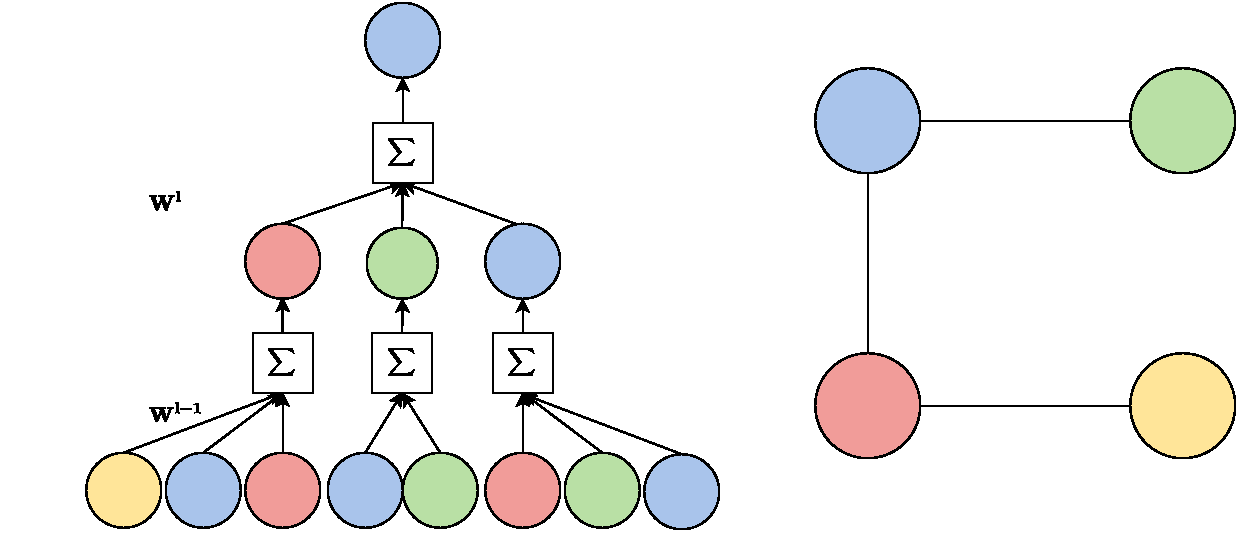
\includegraphics[width=0.8\textwidth]{img/nodecomputationgraph.drawio (5).pdf}
    \caption[Computational graph for computing a node representation]{Exemplary two-layer computational graph for computing the node representation of the blue node in a Graph Neural Network, including self loops.}
    \label{fig:compgraph}
\end{figure}

The GCN formulates the aggregation on a global level, whereby in each step, all node representations are computed taking into account all representations of their neighboring nodes from the previous step. \textcite{hamilton2017inductive} built upon the node-centric view shown in Equation \eqref{eq:matrix_mult2} in practice,  where each node creates its own computational graph (Figure \ref{fig:compgraph}). This allows training the GraphSAGE model using stochastic gradient descent with sampled mini-batches of target nodes and the nodes contained in the target nodes' computational graph. The apporach drastically reduces computational cost and enables training on large scale graphs. Further, they select neighbors randomly to reduce computational cost and empirically find for their usecase a neighborhood size of 25 one-hop and $25\cdot10$ two-hop neighbors to exhibit good performance considering the computational cost. In the present work the notion of node-centric training is utilized and the empirical neighborhood sizes are taken as reference.

Besides computational considerations, the selection of a subset of neighbors is also required for the following reason. By the way the GCN is formulated, for each added layer of the GCN, the receptive field size grows approximately by the power of the average degree. For a large layer count, the target nodes representation is computed by taking into consideration a large amount of other nodes in the graph. For the aggregation architectures introduced until now, the phenomenon known as “over-smoothing” problem \parencite{rusch2023survey} is augmented by increasing the layer count of the GNN. With increasing depth the networks is unable to compute distinguishable node representations for different nodes anymore. The Graph Attention Network aims to reduce this phenomenon.



\begin{equation}
\begin{aligned}
\tilde{\alpha}_{st} &= \mathbf{a}^T [\mathbf{W}h_{s}, \mathbf{W}h_{t}] \\
\alpha_{st} &= \frac{\exp\left(\sigma(\tilde{\alpha}_{st})\right)}{\sum_{u \in \mathcal{N}(t)} \exp\left(\sigma(\tilde{\alpha}_{ut})\right)} \\
h_t' &= \sigma\left(\sum_{s\in \mathcal{N}(t)} \alpha_{st}\mathbf{W}h_{s}\right)
\label{eq:gat}
\end{aligned}
\end{equation}




The \textbf{Graph Attention Network} (GAT) \parencite{velivckovic2017graph} introduces the attention mechanism \parencite{bahdanau2014neural} to GNNs in order to mitigate  the over-smoothing problem. The attention mechanism \eqref{eq:gat} allows the GAT to “attend” to each neighbor $j$ differently by the single scalar $\alpha_{st}$, instead of aggregating each neighbor with equal weight. Therefore, the GAT can selectively choose neighbors it deems as important with respect to computing the target nodes next-layer representation, and diminish the signal of the other nodes, whereby the oversmoothing problem is reduced. Notably, only a single attention vector $\mathbf{a}$ is learned to reduce overfitting on small datasets. In Equation \eqref{eq:gat}, the use of "$[]$" denotes concatenation.  To stabilize the learning process they further concatenate multiple attention heads to learn the final representation ${h_t}$.












 